\chapter{Local Control}
\label{chap:local_control}

The previous chapter presented multiple models that approximate the effects of gripper motion on the deformable object. Next we introduce controllers that use these models to as part of our framework for performing a broad range of tasks.

The role of the local controller is not to perform the whole task, but rather to refine the configuration of the deformable object locally. For our local controller we use a controller of the form introduced in \cite{Berenson2013} and \cite{McConachie2018}. These controllers locally minimize error while avoiding robot collision and excessive stretching of the deformable object. We present two different methods for addressing overstretch in sections \ref{sec:stretching_avoidance_controller} and \ref{sec:stretching_constraint_controller}. Both of these controllers rely on the same method for computing the direction to move the deformable object in order to reduce task error.

\section{Problem Statement}
\todoin{Added max stretch factor $\stretchmax$ to task definition/somewhere - used differently in different controllers. - need to redfined to not be an absolute value but rather a `this is when to get concerned'.}

We define a task based on a set of $\ntargetpoints$ target points $\target \in \targetCspace$, a function $\ErrorFnFull \geq 0$, which measures the alignment error between $\deformconfig$ and $\target$, and a termination function $\TermCondFull$ which indicates if the task is finished. The methods we present in this chapter are local, i.e. at each time $t$ they choose an incremental movement $\grippervel_t$ which reduces the alignment error as much as possible at time $t+1$:
\begin{equation}
    \min_{\grippervel_t} \ErrorFn \left(\target, \deformconfig_{t+1} \right)
    \label{eqn:ctrl_obj}
\end{equation}
where $\deformconfig_{t+1}$ is the result of executing $\grippervel_t$ for one unit of time. $\robotvel_t$ must also be feasible, i.e. it should not bring the grippers into collision with obstacles and should not cause the object to stretch excessively. We will show that several practical tasks can be represented as instances of this problem.

%%%%%%%%%%%%%%%%%%%%%%%%%%%%%%%%%%%%%%%%%%%%%%%%%%%%%%%%%%%%%%%%%%%%%%%%%%%%%%%%%%%%%%%%%%%%%%%%%%%%%%%%%%%%%%%%%%%%%%%

\section{Reducing Task Error}
\label{sec:reducing_error}

\begin{figure}[t]
    \centering
    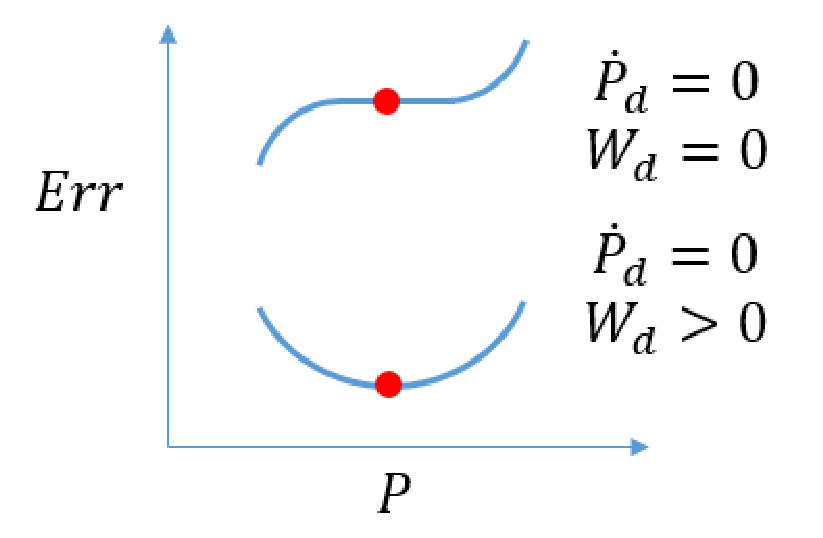
\includegraphics[width=1.8in]{error_graphs_modified}
    \caption{Top Line: moving the point does not change the error, thus the desired movement is zero, however, it is not important to achieve zero movement, thus $\Pinvweight_d = 0$.  Bottom Line: error is at a local minimum; thus moving the point increases error.}
    \label{fig:error_examples}
\end{figure}

\begin{algorithm}[t]
\caption{CalculateCorrespondences$(\deformconfig, \target)$}
\begin{algorithmic}[1]
    \State $\correspondences = [ \emptyset ]_{1 \times \ndeformpoints}$
    \For {$\targetidx \in \{ 1, 2, \dots, \ntargetpoints \}$}
        \State $\deformidx \gets \argmin_{j \in \{ 1, 2, \dots, \ndeformpoints \}} d_\textrm{Dijkstras}(\targetK, \deformconfigJ)$
        \State $d \gets d_\textrm{Dijkstras}(\targetK, \deformconfigI)$
        \State $\correspondences[\deformidx] \gets \{ \correspondences[\deformidx] \cup (\targetidx, d)\}$
    \EndFor
    \State \Return $\correspondences$
\end{algorithmic}
\label{alg:calculate_correspondences}
\end{algorithm}

\begin{algorithm}[t]
\caption{FollowNavigationFunction$(\deformconfig, \correspondences)$}
\begin{algorithmic}[1]
    \State $\deformvel_e \gets \zero_{\deformCspacesize \times 1}$
    \State $\Pinvweight_e \gets \zero_{\ndeformpoints \times 1}$
    \For {$\deformidx \in \{ 1, 2, \dots, \ndeformpoints \}$}
        \For {$(\targetidx, d) \in \correspondences[\deformidx]$}
            \State $\deformvelIpre{e} \gets \deformvelIpre{e} +$ DijkstrasNextStep$(\deformconfigI, \targetidx)$ \label{alg:follow_nav:accumulate}
            \State $\PinvweightIpre{e} \gets \max(\PinvweightIpre{e}, d)$ \label{alg:follow_nav:max}
        \EndFor
    \EndFor
    \State \Return $\deformvel_e, \Pinvweight_e$
\end{algorithmic}
\label{alg:follow_nav_function}
\end{algorithm}

We build on previous work~\cite{Berenson2013}, splitting the desired deformable object movement into two parts: an error correction part and a stretching correction part. When defining the direction we want to move the deformable object to minimize error we calculate two values; which direction to move the deformable object points $\deformvel_e$ and the importance of moving each deformable object point $\Pinvweight_e$. This is analogous to computing the gradient of error, as well as an ``importance factor'' for each part of the gradient. We need these weights to be able to differentiate between points of the object where the error function is a plateau versus points where the error function is at a local minimum~(Fig.~\ref{fig:error_examples}). Typically this is achieved using a Hessian, however our error function does not have a second derivative at many points. 

In order to calculate $\deformvel_e$ and $\Pinvweight_e$, we start by defining a workspace navigation for each target point $\targetK \in \target$ towards $\targetK$ using Dijkstra's algorithm. This gives us the shortest collision-free path between any point in the workspace and the target point, as well as the distance travelled along that path. Using these distances, at every timestep we for every target point $\targetK$, we recalculate which point on the deformable object $\deformconfigI$ is closest (Alg.~\ref{alg:calculate_correspondences}). The directions each navigation function indicates are added together to define the overall direction to manipulate a point (Alg.~\ref{alg:follow_nav_function} line \ref{alg:follow_nav:accumulate}). For the importance factors $\Pinvweight_{e,\deformidx}$, we take only the largest distance that $\deformconfigI$ would have to move as a way to mitigate discretization effects (Alg.~\ref{alg:follow_nav_function} line \ref{alg:follow_nav:max}).

%%%%%%%%%%%%%%%%%%%%%%%%%%%%%%%%%%%%%%%%%%%%%%%%%%%%%%%%%%%%%%%%%%%%%%%%%%%%%%%%%%%%%%%%%%%%%%%%%%%%%%%%%%%%%%%%%%%%%%%

\section{Stretching Avoidance Controller}
\label{sec:stretching_avoidance_controller}

\begin{algorithm}[ht]
    \caption{StretchingAvoidanceController$(\gripperconfig, \deformconfig, \target)$}
    \begin{algorithmic}[1]
        \State $\correspondences \gets$ CalculateCorrespondences$(\deformconfig, \target)$
        \State $\deformvel_e, \Pinvweight_e \gets$ FollowNavigationFunction$(\deformconfig, \correspondences)$
        \State $\deformvel_s, \Pinvweight_s \gets$ StretchingCorrection$(\deformconfig)$
        \State $\deformvel_d, \Pinvweight_d \gets$ CombineTerms$(\deformvel_e, \Pinvweight_e, \deformvel_s, \Pinvweight_s)$
        \State $\grippervel \gets$ FindBestRobotMotion$(\gripperconfig, \deformconfig, \deformvel_d, \Pinvweight_d)$
    \end{algorithmic}
    \label{alg:stretching_avoidance_controller}
\end{algorithm}

An outline of how this controller functions is shown in Alg.~\ref{alg:stretching_avoidance_controller}; first, we calculate the error reduction direction and weight as discussed in the previous section (Lines 1 and 2). These error reduction terms are then combined with stretching avoidance terms $\deformvel_s, \Pinvweight_s$ to define the desired manipulation direction and importance weights $\deformvel_d, \Pinvweight_d$ at each timestep (Lines 3 and 4). We then find the best robot motion to achieve the desired deformable object motion, while preventing collision between the robot and obstacles (Line 5).

\subsection{Stretching Correction}
\label{sec:stretching_correction}

\begin{algorithm}[ht]
\caption{StretchingCorrection$(\deformconfig)$}
\begin{algorithmic}[1]
    \State $E \gets$ EuclidianDistanceMatrix$(\deformconfig)$
    \State $\deformvel_s \gets \zero_{\deformCspacesize \times 1}$
    \State $\Pinvweight_s \gets \zero_{\ndeformpoints \times 1}$
    \For{$\deformidx \in \{1,2,\dots,\ndeformpoints \}$}
        \For{$j \in \text{Neighbours}(i)$}
            \If{$\deformidx < j$ \textbf{and} $E_{\deformidx j} > \stretchmax \geodistIJ$}
                \State $\Delta_{\deformidx j} \gets E_{\deformidx j} - \geodistIJ$
                \State $v \gets \Delta_{\deformidx j}(\deformconfigJ - \deformconfigI)$
                \State $\deformvelIpre{s} \gets \deformvelIpre{s} + \frac{1}{2}v$
                \State $\deformvelJpre{s} \gets \deformvelJpre{s} - \frac{1}{2}v$
                \State $\PinvweightIpre{s} \gets \max (\PinvweightIpre{s}, \Delta_{\deformidx j})$
                \State $\PinvweightJpre{s} \gets \max (\PinvweightJpre{s}, \Delta_{\deformidx j})$
            \EndIf
        \EndFor
    \EndFor
    \State \Return $\deformvel_s, \Pinvweight_s$
\end{algorithmic}
\label{alg:stretching_correction_ijrr}
\end{algorithm}

\begin{algorithm}[ht]
\caption{CombineTerms$(\deformvel_e, \Pinvweight_e, \deformvel_s, \Pinvweight_s)$}
\begin{algorithmic}[1]
    \For{$\deformidx \in \{ 1,2,\dots,\ndeformpoints \}$}
        \State $\deformvelIpre{d} \gets \deformvelIpre{s} + \left( \deformvelIpre{e} - \proj_{\deformvelIpre{s}} \deformvelIpre{e} \right)$
        \State $\PinvweightIpre{d} \gets \stretchweightfactor \PinvweightIpre{s} + \PinvweightIpre{e}$
    \EndFor
    \State \Return $\deformvel_d, \Pinvweight_d$
\end{algorithmic}
\label{alg:combine_terms}
\end{algorithm}


Our algorithm for stretching correction is similar to that found in~\cite{Berenson2013}, with the addition of a weighting term $\stretchweightfactor$, and a change in how we combine error correction and stretching correction. We use the StretchingCorrection() function (Alg.~\ref{alg:stretching_correction_ijrr}) to compute $\deformvel_s$ and $\Pinvweight_s$ based on a task-defined stretching threshold $\Pinvweight_s \geq 0$. First we compute the distance between every two points on the object and store the result in $E$. We then compare $E$ to $\geodist$ which contains the relaxed lengths between every pair of points. If any two neighbouring points are stretched by more than a factor of $\Pinvweight_s$, we attempt to move the points closer to each other. We use the same strategy for setting the importance of this stretching correction $\Pinvweight_s$ as we use for error correction. When combining stretching correction and error correction terms (Alg.~\ref{alg:combine_terms}) we prioritize stretching correction, accepting only the portion of the error correction that is orthogonal to the stretching correction term for each point. $\stretchweightfactor$ is used to define the relative scale of the importance factors $\Pinvweight_e$ and $\Pinvweight_s$


\subsection{Finding the Best Robot Motion}

\todoin{Cleanup $\JacobianFull$ vs $J$ vs $J_d$ vs $J_r$ in this section.}

Given a desired deformable object velocity $\deformvel_d$ and relative importance weights $\Pinvweight_d$, we want to find the robot motion that best achieves $(\deformvel_d, \Pinvweight_d$). I.e.
\begin{equation}
\begin{aligned}
    & \argmin_{\robotvel} 
        & & \| \DeformForwardFnFull - \deformvel_d \|_{\Pinvweight_d} \\
    & \text{subject to}
        & & \| \robotvel \| \leq \robotvelmax \\
    &   & & \left(\robotconfig + \robotvel \right) \in \robotCvalid \enspace .
\end{aligned}
\label{eqn:controller_minimization_problem_apx}
\end{equation}
In general, $\DeformForwardFn(\dots)$ is not known. For our stretching avoidance controller we use a Jacobian based approximation (Chapter.~\ref{chap:modelling}):
\begin{equation}
    \DeformForwardFnFull \approx \JacobianFull \robotvel
\end{equation}
Our method for ensuring the robot stays in $\robotCvalid$ is different, depending on which robot we are using.

\subsubsection{Simulated experiments:}

For the simulated experiments, we first solve Eq.~\eqref{eqn:controller_minimization_problem_apx} using our Jacobian approximation while neglecting the collision constraints:
\begin{equation}
\begin{aligned}
    \DeformBackwardFn_{\tanse3}(\deformvel, \Pinvweight) =
        &\argmin_{\grippervel }
            & & \| J \grippervel - \deformvel \|_{\Pinvweight} \\
        &\textrm{subject to}
            & & \grippervelGnorm \leq \grippervelmaxservo \enspace, \quad \gripperidx = 1, \dots, \ngrippers
    \label{eqn:jacobianbackwardfunction_sim}
\end{aligned}
\end{equation}
where $\grippervelmaxservo$ is the maximum velocity for each individual gripper.
% (Alg.~\ref{alg:find_best_robot_motion_simulation}).

In order to guarantee that the grippers do not collide with any obstacles, we use the same strategy from~\cite{Berenson2013}, smoothly switching between collision avoidance and other objectives (see Alg.~\ref{alg:obstaclerepulsion}). For every gripper $\gripperidx$ and an obstacle set $\obstacle$ we find the distance $d_\gripperidx$ to the nearest obstacle, a unit vector $\dot x_{p_\gripperidx}$ pointing from the obstacle to the nearest point on the gripper, and a Jacobian $J_{p^\gripperidx}$ between the gripper's DoF and the point on the gripper as shown in Alg.~\ref{alg:proximity}. We then project the servoing motion from Eq.~\eqref{eqn:jacobianbackwardfunction_sim} into the null space of the avoidance motion using the null space projector $\left(\eye - J_{p^g}^+ J_{p^g} \right)$. $\obsavoidfactor > 0$ sets the rate at which we change between servoing and collision avoidance objectives. $\grippervelmaxobs > 0$ is an internal parameter that sets how quickly we move the robot away from obstacles.





\begin{algorithm}[ht]
\caption{FindBestRobotMotionSim$(\gripperconfig, \deformconfig, \deformvel_d, \Pinvweight_d)$}
\label{alg:find_best_robot_motion_simulation}
\begin{algorithmic}[1]
    \State $\grippervelS \gets \DeformBackwardFn_{\tanse3} (\deformvel_d, \Pinvweight_d)$ \hfill Eq.~\eqref{eqn:jacobianbackwardfunction_sim}
    \State $\grippervelcmd \gets $ ObstacleRepulsion$(\grippervelS, \obstacle)$
    \State \Return $\grippervelcmd$
\end{algorithmic}
\end{algorithm}

\todoin{Clean up inputs etc. - $q$ is needed for repulsion, proximity etc.}

\begin{algorithm}[ht]
\caption{ObstacleRepulsion$(\grippervelS, \obstacle)$}
\begin{algorithmic}[1]
    \For{$\gripperidx \in \{1, \dots, \ngrippers \}$}
        \State $J_{p^\gripperidx}, \dot x _{p^\gripperidx}, d_\gripperidx \gets$ Proximity$(\gripperconfigG, \obstacle)$
        \State $\lambda \gets e^{-\obsavoidfactor d_\gripperidx}$
        \State $v \gets J_{p^\gripperidx}^+ \dot x_{p^\gripperidx}$
        \State $\grippervelGC \gets \grippervelmaxobs \frac{v}{\| v \|}$
        \State $\grippervelG \gets$ $\lambda \left( \grippervelGC + \left( \eye - J_{p^\gripperidx}^+ J_{p^\gripperidx} \right) \grippervelGS \right) + (1-\lambda) \grippervelGS$
    \EndFor        
    \State \Return $\grippervel$
\end{algorithmic}
\label{alg:obstaclerepulsion}
\end{algorithm}


\begin{algorithm}[ht]
\caption{Proximity$(\gripperconfigG, \obstacle)$}
\label{alg:proximity}
\begin{algorithmic}[1]
    \State $d_\gripperidx \gets \infty$
    \For{$o \in \{1,2,\dots,|\obstacle|\}$}
        \State $p^\gripperidx, p^o \gets$ ClosestPoints$(\gripperconfigG, o)$
        \State $v \gets p^\gripperidx - p^o$
        \If{$\| v \| < d_\gripperidx$}
            \State $d_\gripperidx \gets \| v \|$
            \State $\dot x_{p^\gripperidx} \gets \frac{v}{\| v \|}$
            \State $J_{p^\gripperidx} \gets$ RobotPointJacobian$(\gripperconfigG, p^\gripperidx)$
        \EndIf
    \EndFor
    \State \Return $J_{p^\gripperidx}, \dot x_{p^\gripperidx}, d_\gripperidx$
\end{algorithmic}
\end{algorithm}


\subsubsection{Physical experiments:}
\label{sec:stretching_avoidance_controller_physical_robot_implementation}

\todoin{Clean up $J_{p^g}$ vs $J_{c_i}$ etc. throughout this section. And $J_d, J_r$.}

\begin{algorithm}[ht]
\caption{FindBestRobotMotionPhys$(\gripperconfig, \deformconfig, \deformvel_d, \Pinvweight_d)$}
\label{alg:find_best_robot_motion_physical}
\begin{algorithmic}[1]
    \For {$\gripperidx \in \{ 1, 2, \dots, | \mathcal{C} | \}$}
        \State $J_{p^\gripperidx}, \dot x _{p^\gripperidx}, d_\gripperidx \gets$ Proximity$(\obstacle, \gripperidx)$
    \EndFor
    \State $\robotvelcmd \gets \DeformBackwardFn_{\physrobotVspace} (\deformvel_d, \Pinvweight_d)$ \hfill Eq.~\eqref{eqn:jacobianbackwardfunction_live}
\end{algorithmic}
\end{algorithm}

For the physical robot, instead of handling collision avoidance in a post-processing step, we build the collision constraints directly into the optimization function (Alg.~\ref{alg:find_best_robot_motion_physical}). To do so, we define a set of points  $\mathcal{C} = \{c_1, c_2, \dots \}$ on the robot that must stay at least $\dbuffer$ away from obstacles. In our implementation, this is the end-effectors, wrists, and elbows of each arm of the robot. We then use the same Proximity() function\todo{it's not quite the same} (Alg.~\ref{alg:proximity}) as the simulated robot to define an extra constraint that must be satisfied:
\begin{equation}
\begin{aligned}
    \DeformBackwardFn_{\reals^N}(\deformvel, \Pinvweight) = 
        &\argmin_{\robotvel}    & & \| J_d \grippervel - \deformvel \|^2_{\Pinvweight} \\
        &\text{subject to}      & & \hspace{1.2cm} \llap{$\robotconfig + \robotvel$} \in \robotCvalid \\
        &                       & & \hspace{1.2cm} \llap{$\| \robotvel \|$}          \leq \physrobotvelmax \\
        &                       & & \hspace{1.2cm} \llap{$\| J_{r,\gripperidx} \robotvel \|$}  \leq \grippervelmaxservo \enspace , \quad g = 1, \dots, \ngrippers \\
        &                       & & \hspace{1.2cm} \llap{$\dot x_{c_i}^T J_{c_i} \grippervel$} \leq d_{c_i} + \dbuffer \enspace , \quad i = 1, \dots, |\mathcal{C}| \enspace .
\label{eqn:jacobianbackwardfunction_live}
\end{aligned}
\end{equation}
In addition, we constrain the velocity of the robot both in joint configuration space 
$$ \| \grippervel \| \leq \physrobotvelmax $$
and the velocity of the end-effectors in $\se3$ 
$$ \| J_{r,\gripperidx} \grippervel \| \leq \grippervelmaxservo $$
where $J_{r,\gripperidx}$ is the Jacobian between robot motion and end effector motion for gripper $\gripperidx$.

To solve Equations \eqref{eqn:jacobianbackwardfunction_sim} and \eqref{eqn:jacobianbackwardfunction_live} we use the Gurobi optimizer (\cite{Gurobi2016}). Table~\ref{tab:controller_param_table} shows the parameters we use for each experiment.

%%%%%%%%%%%%%%%%%%%%%%%%%%%%%%%%%%%%%%%%%%%%%%%%%%%%%%%%%%%%%%%%%%%%%%%%%%%%%%%%%%%%%%%%%%%%%%%%%%%%%%%%%%%%%%%%%%%%%%%

\section{Stretching Constraint Controller}
\label{sec:stretching_constraint_controller}

\todoin{Update notation throughout - including figures}
\todoin{Make algorithm block}

% \begin{algorithm}[ht]
%     \caption{LocalConstrainedController$(\robotconfig, \deformconfig, \deformtarget, \relaxeddistancematrix, \stretchmax)$}
%     \begin{algorithmic}[1]
%         \State $\correspondences \gets$ CalculateCorrespondences$(\deformconfig_t, \deformtarget)$
%         \State $\deformvel_e, \Pinvweight_e \gets$ FollowNavigationFunction$(\deformconfig_n, \correspondences)$
%         \State $\robotcommandvel \gets$ FindBestConstrainedRobotMotion$(\robotconfig, \deformconfig, \deformvel_e, \Pinvweight_e)$
%     \end{algorithmic}
%     \label{alg:local_constrained_controller}
% \end{algorithm}

While the controller in the previous section has had some success at preventing excessive stretching~\cite{Berenson2013}, it is not able to prevent stretching when the grippers move on opposite sides of an obstacle (see attached video). To address this, we introduce a novel geometric constraint which is able to directly address the cause of overstretch.

\subsection{Overstretch}
\label{Method_Overstretch}
The stretching avoidance of the deformable object is formulate due to the compliant nature and the lack of control of the deformable object. In the previous section, a stretching correction term $\deformvel_s \in \deformVspace$ is applied when the object becomes overstretched. However, this method cannot handle cases where the object is caught on an obstacle.

We detect the overstretching (i.e. excessive strain) of the object by examining the value of the stretching ratio $\stretchcurr$, which denotes the maximum value among the ratio between the Euclidean distance $\| \straightvecIJ \|$ and the geodesic distance $\geodistIJ$ for every pair of points $\deformconfigI$ and $\deformconfigJ$:
\begin{equation}
    \stretchcurr = \max_{\substack{\deformidx, j \in 1, \dots, \ndeformpoints \\ j > \deformidx}} \frac{\| \straightvecIJ \|}{\geodistIJ}
    \label{Eq:Method_stretching_detection}
\end{equation}
we denote $\stretchmax$ as the maximum allowed stretching ratio. Our method initiates stretching-avoidance when $\stretchcurr > \stretchmax$.
\todoin{we've already defined $\stretchmax$ earlier.}

We assume that the object starts in an unstretched state, so the overstretch that arises is due to the motion of the grippers. Thus if we can constrain gripper motions to a set which does not overstretch the object further than a threshold, we can prevent or reduce the overstretch at the next time step. We know that the force causing the overstretch comes from the grippers, so if we reduce the length of geodesic paths through the object between grippers, the strain on the object should decrease. When overstretch is detected, we thus introduce a conical constraint for each gripper that shrinks the allowable $\grippervelG$ to reduce the length of the geodesics between the grippers. 

\begin{figure}[ht]
    \centering
    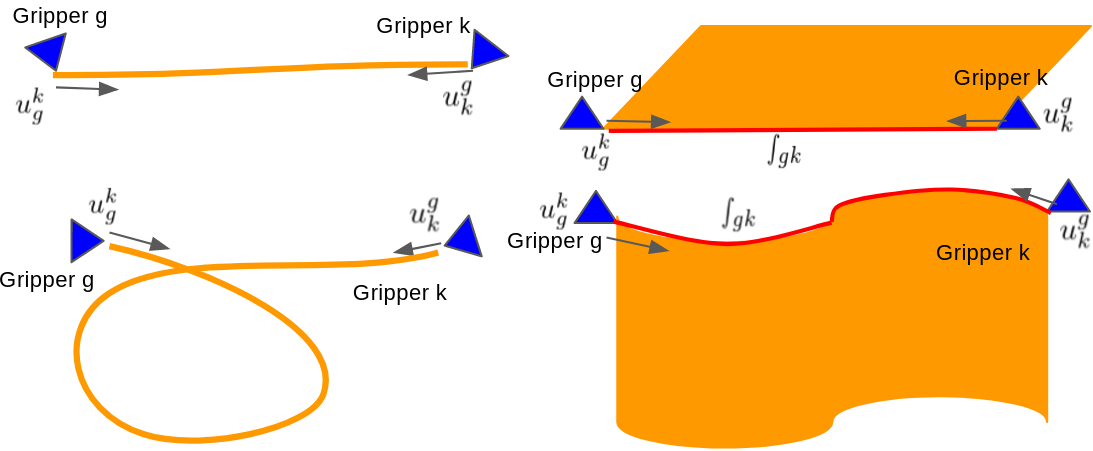
\includegraphics[width=.98\linewidth]{Stretching_vector_method.png}
    \caption{The arrows in gray show the direction of each stretching vector at the corresponding gripper with respect to the gripper pair $\gripperconfigG$ and $\gripperconfigK$. Left: stretching vectors on the rope when the rope is at rest (above) or is deformed (below). Right: stretching vectors on the cloth when the cloth is at rest (above) or is deformed (below). The red lines denote the geodesic connecting the corresponding $\deformconfigGK$ and $\deformconfigKG$ on the object.}
    \label{Fig:stretching_avoidance_vector_method}
\end{figure}

A conical constraint is constructed for each gripper and points along the \textit{stretching avoidance vector}, which is an estimation of the direction to move to decrease the strain. For a pair of grippers with index $\gripperidx$ and $k$, two stretching avoidance vectors are defined, one for each gripper. Let $\closestpointGK$ be the index of the point grasped by the $\gripperidx$th gripper, which has the minimum geodesic distance to the set of points grasped by $\gripperconfigK$. We define $\closestpointKG$ similarly.  Let $\geodesicGK$ be the geodesic on the object from $\deformconfigGK$ to $\deformconfigKG$. We denote $\savoidGK$ and $\savoidKG$ as the pair of stretching avoidance vectors on grippers $\gripperidx$ and $k$ respectively.  Then $u^k_g$ is the tangent vector of $\geodesicGK$ at $\deformconfigGK$ and $\savoidGK$ is the tangent vector of $\geodesicKG$ at the point $\deformconfigKG$ (as shown in Fig. \ref{Fig:stretching_avoidance_vector_method}). 

\todoin{Go through and revise notation for $C_s$ and $s$ etc.}

To specify the stretching constraint, we first define the function $s(\grippervelG, \gripperconfigG, \gripperconfigK, \deformconfig)$, which specifies the constraint on gripper $\gripperidx$ defined by the interaction of grippers $\gripperidx$ and $k$. Correspondingly, $\savoidGK$ is the stretching avoidance vector for gripper $\gripperidx$, which is the tangent vector of $\geodesicGK$ at $\deformconfigGK$. The larger the value of $s$, the more we expect geodesic path length between grippers will be reduced. Thus, $s$ should increase as $\angle (\grippervelG, \savoidGK)$ increases. Assume we wish to have a lower bound $s_s$ on $s$, then $C_s$ is a set of constraints $C_s = \{C_s^1, \dots, C_s^G\}$, where each constraint is:
\begin{equation}
    C_s^g =\{ \grippervelG\in \tanse3 \mid \forall k\neq g, \ s(\grippervelG, \gripperconfigG, \gripperconfigK, \deformconfig) \geq s_s  \}
    \label{Eq:Stretching_avoidance_Method}
\end{equation}
Many functions can satisfy the requirements of $s$. In our work, we specify the function as:
\begin{equation}
    s(\grippervelG, \gripperconfigG, \gripperconfigK, \deformconfig) = \cos \angle (\grippervelG, \savoidGK ) = \cos \angle (\transvelG, \savoidGK )
    \label{Eq:Stretching_avoidance_Method_This_Paper}
\end{equation}

\subsection{Collision} Collision avoidance for the robot is addressed by the constraint $C_c$, which is the set of motions that keeps the grippers away from obstacles:

\todoin{Replace this with reference to Proximity etc earlier}

\begin{equation}
    C_c = \left\{\grippervelG\in \tanse3 \mid  \dbuffer - l(\gripperconfigG) - \frac{\mathfrak{n}(\gripperconfigG) \cdot \grippervelG}{||\grippervelG||} \grippervelG \Delta t < 0\right\}
    \label{Eq:Collision_constraint_Method}
\end{equation}
where $l(\gripperconfigG)$ is the function returning the distance from the gripper to its closest obstacle. $\mathfrak{n}(\gripperconfigG)$ returns the unit surface normal of the obstacle closest to the $\gripperidx$th gripper. The idea is to make each gripper keep at least the safe distance away from the closest obstacle. While we consider free-flying grippers in this section, similar constraints can be imposed on the entire geometry of a robot arm to avoid collisions all along the arm as was done in Sec.~\ref{sec:figureoutwhattorefhere}.


\subsection{Optimization Method}

Given these constraints, we then formulate an optimization problem similar to Eq.~\eqref{eqn:jacobianbackwardfunction_sim}, replacing the approximate Jacobian model with the directional rigidity model (Sec.~\ref{sec:constrained_model}), and adding the new stretching and collision constraints.

\todoin{Replace $C_s$ and $C_c$ with something else more directly accurate}
\todoin{Confirm these max vel equations in the implementation}

\begin{equation}
\begin{aligned}
    \DeformBackwardFn(\deformvel, \Pinvweight) = 
        & \argmin{\grippervel}
            & & \| \DeformForwardFnFull - \deformvel_e \|_{\Pinvweight_e} \\
        & \textrm{subject to}
            & & \grippervel \in C_s\\
        &   & & \grippervel \in C_c\\
        &   & & \grippervelGnorm \leq \grippervelmaxservo \enspace, \quad \gripperidx = 1, \dots, \ngrippers
\end{aligned}
\label{Eq:Optimization Problem}
\end{equation}

Because our objective function is not necessarily convex, we used a custom optimization method to solve the problem specified in Eq. \ref{Eq:Optimization Problem}. Our method is a type of numerical gradient descent with an additional projection step to enforce constraints.

Our method's outer loop computes the numerical gradient of the objective function. An inner loop then performs backtracking line search to find the gradient step size. However, the gradient step may cross a constraint boundary, thus after we compute the step size, we check if any constraint has been violated after taking the step. If it has, we project the step back to the feasible space. A simple projection to the boundary of a violated constraint may satisfy that constraint but violate others. Instead, to perform the projection, we solve a convex optimization problem (using the Gurobi optimizer \cite{Gurobi2016}) to find the nearest feasible point. This is possible because all the constraints in our problem are convex. Once such a point is found, the outer loop continues to iterate until convergence.

%%%%%%%%%%%%%%%%%%%%%%%%%%%%%%%%%%%%%%%%%%%%%%%%%%%%%%%%%%%%%%%%%%%%%%%%%%%%%%%%%%%%%%%%%%%%%%%%%%%%%%%%%%%%%%%%%%%%%%%

\subsection{Results}
\label{sec:stretching_constraint_controller_results}

Our goal for this new controller is formulating a set of constraints for the controller to mitigate collision and excessive stretching issues. As mentioned in previous sections, our benchmark controller is based on \cite{Berenson2013} and described in Sec.~\ref{sec:stretching_avoidance_controller}. To evaluate our method we perform experiments in simulation and on a physical robot. The simulator used is Bullet physics \cite{Coumans2010}, however, we emphasize that our method has no knowledge of the simulation parameters or simulation methods used therein. The simulator is used as a ``black-box,'' mainly to stand in for a perception system and to allow us to do repeatable experiments. The physical robot consists of two KUKA iiwa 7DoF arms with Robotiq 3-finger hands.

\todoin{Separate text/wording etc. for model vs controller.}

We ran experiments with scenarios involving both cloth and rope. The parameters are set as $\drkdir = 4$, $\drkdist = 10$, $\drkrot = 20$ for the new model, $l_c = 0.023$, and $s_s = 0.4$ for the new controller. The parameters we used for the benchmark method are its default best value found in \cite{McConachie2018}. The stretching detection ratio is set as $\stretchmax = 1.667$ for the cloth and $\stretchmax = 1.1$ for the rope. The maximum gripper motion is set as $grippervelmaxservo = 0.2$. For the experiment with a task goal defined, a precalculated Dijkstra field for the task will generate the $\deformvel_e$ for each point at each state to move the object toward the goal given each point's current position in the space as described in Sec.~\ref{sec:reducing_error}. All experiments were run on a i7-8700K 3.7 GHz CPU with 32 GB of RAM. A video showing the experiments is included with this paper.


\subsection{Constraint Enforcement}
\label{Results: Object Stretching Avoidance}

Since the benchmark controller can already handle the collision constraint very well, and the new controller addresses the collision constraint in the similar way as the benchmark, there is not a significant difference in how the collision constraint is enforced. However, the stretching constraint shows a very clear improvement.

The metrics of stretching avoidance is the stretching ratio $\stretchcurr$ defined in Section \ref{Method_Overstretch}. A controller with good stretching avoidance should prevent $\stretchcurr$ from increasing beyong a certain threshold.

The two experiments we used for the stretching avoidance test are the rope-wrapping-cylinder and the cloth-passing-single-pole, shown in Fig.\ref{fig:experimental_setup_scene} (left column). We ran each controller separately for a fixed amount of time for each task and show $\stretchcurr$ vs. time for both controllers in Fig. \ref{fig:experiment_stretching_factorFig: experiment_stretching_factor}. In both these two setups, the desired object motion $\deformvel_e$ generated by the Dijkstra field will tear the object unless overstretching is prevented.%, thus the 

Fig. \ref{fig:experiment_stretching_factorFig: experiment_stretching_factor} shows the new controller is able to prevent further stretching happening when the object is taut for both the rope and the cloth. In the rope test, the new controller can prevent overstretching with $s_s = 0.4$, as defined in Eq.\ref{Eq: Stretching_avoidance_Method_This_Paper}. We can see the $\stretchcurr$ of the benchmark methods keeps growing beyond this threshold, while the $\stretchcurr$ of the new method stays close to the threshold. In the cloth test, the benchmark method's $\stretchcurr$ (in purple) increases above the threshold $\stretchmax = 1.667$ for cloth, and a sudden drop in $\stretchcurr$ happens after running the test for $2$ seconds. This drop is the ``tearing'' point in the simulator. Though we still see overstretching happened using the new method for some settings of $s_s$, in all cases the $\stretchcurr$ converged before tearing happened (instead of growing without bound). 

\begin{figure}[t]
    \centering
    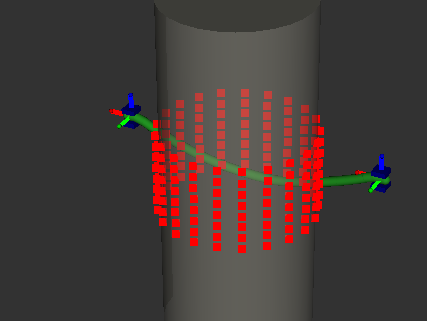
\includegraphics[width=.45\linewidth]{rope_cylinder}\hfill
    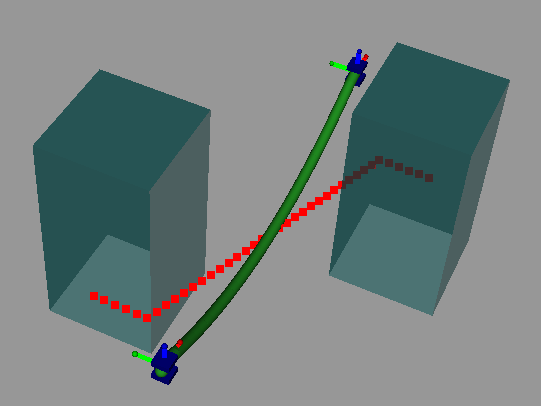
\includegraphics[width=.45\linewidth]{rope_zig_match}\\
    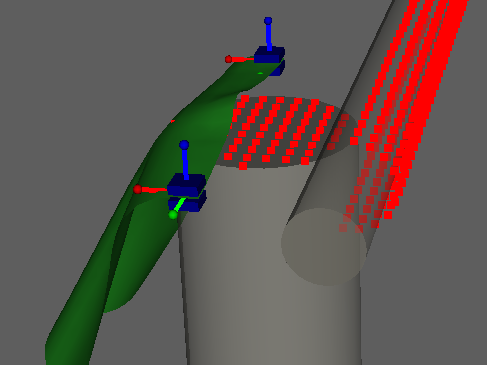
\includegraphics[width=.45\linewidth]{cloth_wafr}\hfill
    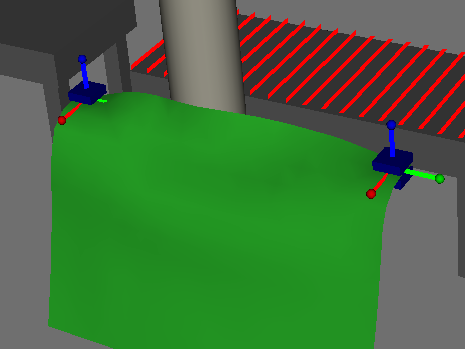
\includegraphics[width=.45\linewidth]{cloth_single_pole}%
    \caption{Initial state of the four experiments, where the red points act as attractors for the deformable object.}
    \label{fig:experimental_setup_scene}
\end{figure}


\begin{figure}[t]
    \centering
    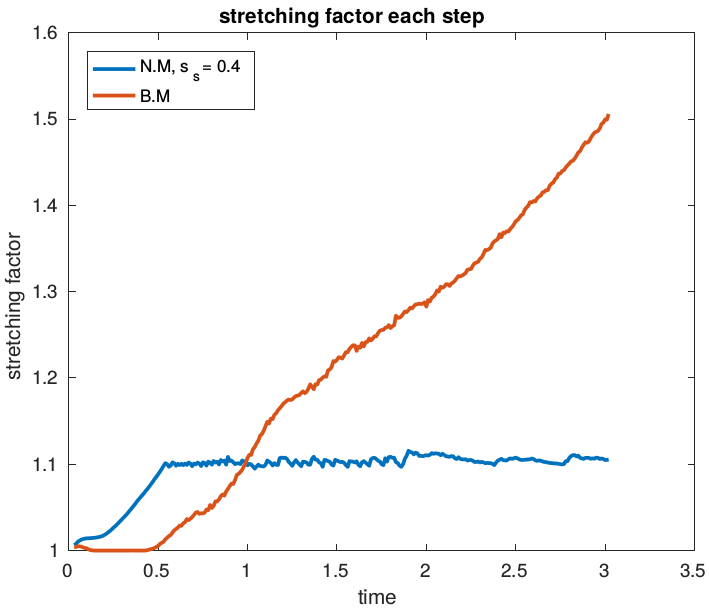
\includegraphics[width=.45\linewidth]{stretching_rope_cylinder} \hfill
    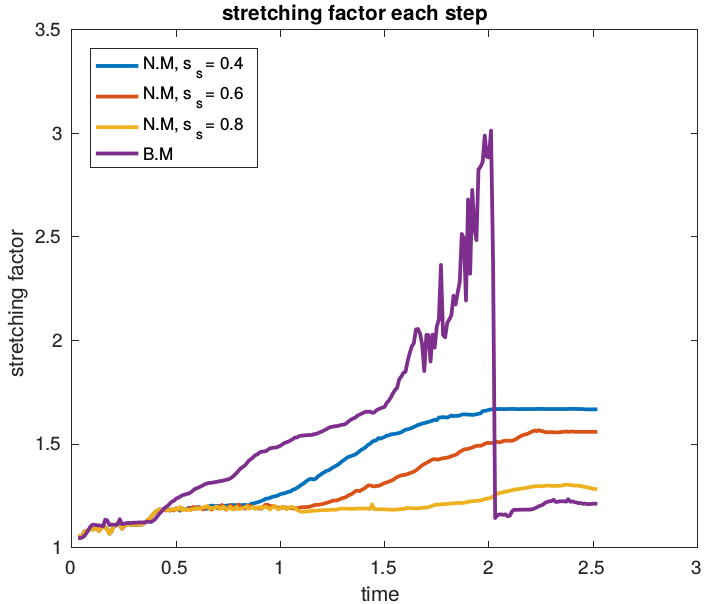
\includegraphics[width=.45\linewidth]{stretching_cloth_single_pole}%
    \caption{Cloth passing single pole}
    \label{Fig: stretching factor scene_cloth_single_pole}
    \caption{(a) The red line shows the $\stretchcurr$ of the benchmark and the blue line shows the $\stretchcurr$ of the new controller with $s_s = 0.4$ throughout the simulation. (b) The purple line shows the $\stretchcurr$ of the benchmark, and the blue, red, and yellow lines each show the $\stretchcurr$ of the new controller with $s_s = 0.4$, $s_s = 0.6$, and $s_s = 0.8$, respectively.}
    \label{fig:experiment_stretching_factorFig: experiment_stretching_factor}
\end{figure}




%We find that setting a tighter constraint, such as increasing the value of $s_s$, can help prevent excessive stretching in the object, as shown in Fig. \ref{Fig: cos_stretching}. 


% Explain the trade-off between constraints avoidance and control accuracy
%Examining Fig. \ref{Fig: experiment_model_error} and Fig. \ref{fig:experiment_stretching_factorFig: experiment_stretching_factor}, we found that when there is no constraints violation detected, the new controller can generally have a smaller control error.
%When the constraints violation happens, the new controller will tend to mitigate this violation and take the trade off in control accuracy.  



\subsection{Controller Task Performance} \label{Results:Controller Task Performance}

Besides the quantitative analysis of the model accuracy and stretching avoidance, we ran another two experiments, rope-matching-zig-path and cloth-covering-two-cylinder, one each with the rope or the cloth, as shown in Fig.~\ref{fig:experimental_setup_scene} to see how the new method performed for some coverage tasks. Both the benchmark and the new controllers are able to perform these tasks with comparable performance; reaching approximately the same configurations when forward progress stops due to a local minimum (Fig.~\ref{fig:cloth_wafr_performance}), and completing the task (Fig.~\ref{fig:zigzeg_performance}). This result suggests that we have not lost functionality with respect to the benchmark despite changing the model and control method used.


\begin{figure}[t]
    \centering
    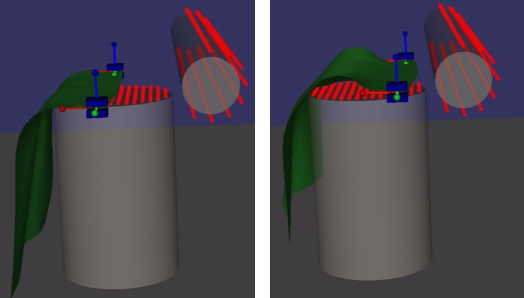
\includegraphics[width=\columnwidth]{cloth_wafr_performance.png}
    \caption{Cloth-covering-two-cylinder task start and end configurations. Both controllers are unable to make progress due to a local minima.}
    \label{fig:cloth_wafr_performance}
\end{figure}


\begin{figure}[t]
    \centering
    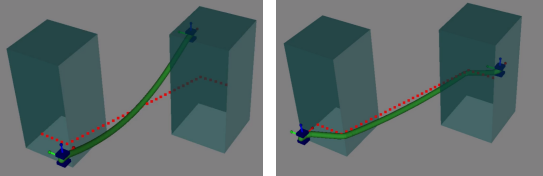
\includegraphics[width=\columnwidth]{zigzeg_performance.png}
    \caption{Rope-matching-zig-path start and end configurations. Both controllers are able to succeed at the task, bringing the rope into alignment with the desired path.}
    \label{fig:zigzeg_performance}
\end{figure}



\subsection{Physical Robot Experiments}

To evaluate our new model and controller on a physical system, we set up an experiment with cloth-like objects manipulated by two 7DoF KUKA iiwa arms (Fig.~\ref{fig:physical_experiment_screenshots_ctl}). To sense the position of the cloth, we use the AprilTags~\cite{olson2011tags} and IAI Kinect2~\cite{iai_kinect2} libraries. The parameters are set as $\drkdir = 4$, $\drkdist = 10$, $\drkrot = 10$ for the new model, $l_c = 0.08$, and $s_s = 0.6$ for the new controller. We set up a task similar to the cloth-passing-single-pole example using a paper towel. For this task, the baseline controller tears the paper towel while the new controller avoids excessive overstretch, instead wrapping around the pole to reach a local minimum.

\begin{figure}[t]
    \centering
    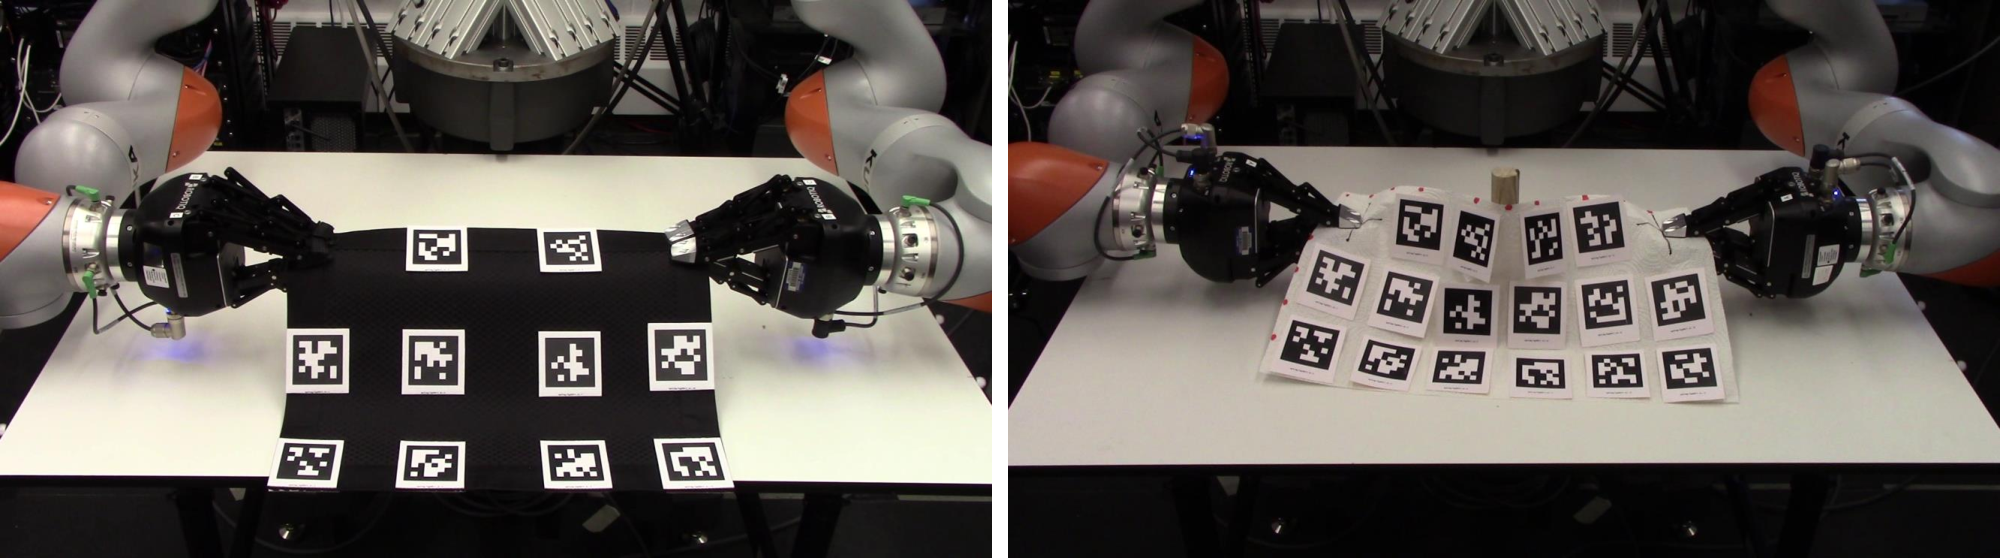
\includegraphics[width=0.85\columnwidth,trim=6.7in 0 0 0,clip]{physical_robot_experiment_screenshots.pdf}
    \caption{Initial setup for the physical robot stretching avoidance test.}
    \label{fig:physical_experiment_screenshots_ctl}
\end{figure}


\subsection{Computation Time}

\begin{table}[t]
\centering
\caption{Mean computation time (s) to compute the gripper motion for a given state. BM: benchmark method; NM: new method.}
\begin{tabular}{lccccc}
\hline
        & \makecell{rope-wrapping\\-cylinder} 
        & \makecell{rope-matching\\-cylinder}
        & \makecell{cloth-passing\\-single-pole}
        & \makecell{cloth-wrapping\\-two-cylinder} \\
BM      & 0.0055   & 0.0054  & 0.0153  & 0.0037   \\ \hline
NM      & 0.0342   & 0.0834  & 0.2363  & 0.1008   \\ \hline
\end{tabular}
\label{tbl:constraint_controller_time_report}
\end{table}

To verify the practicality of our method, we gathered data comparing its computation time to the benchmark's and to using the Bullet simulator. Table~\ref{tbl:constraint_controller_time_report} shows the average computation time of a call to the controller for the new method vs. the benchmark. As expected, the benchmark, which uses a linear model, is faster than the new method. However, the computation times for the new method are still reasonable to use in a control loop.
